\documentclass{beamer}

% Copyright (c) 2022 by Lars Spreng
% This work is licensed under the Creative Commons Attribution 4.0 International License. 
% To view a copy of this license, visit http://creativecommons.org/licenses/by/4.0/ or send a letter to Creative Commons, PO Box 1866, Mountain View, CA 94042, USA.

%~~~~~~~~~~~~~~~~~~~~~~~~~~~~~~~~~~~~~~~~~~~~~~~~~~~~~~~~~~~~~~~~~~~~~~~~~~~~~~
% Add your packages and commands to this file
%~~~~~~~~~~~~~~~~~~~~~~~~~~~~~~~~~~~~~~~~~~~~~~~~~~~~~~~~~~~~~~~~~~~~~~~~~~~~~~

%~~~~~~~~~~~~~~~~~~~~~~~~~~~~~~~~~~~~~~~~~~~~~~~~~~~~~~~~~~~~~~~~~~~~~~~~~~~~~~
\RequirePackage{palatino}
\RequirePackage[utf8]{inputenc}
\RequirePackage[T1]{fontenc}

\usefonttheme{serif}

\usepackage{styles/elegantmacros}
\usefolder{styles}
\usetheme[style=blue]{elegant}

\newcommand{\makepart}[1]{ % For convenience
\part{#1} \frame{\partpage}
}

%~~~~~~~~~~~~~~~~~~~~~~~~~~~~~~~~~~~~~~~~~~~~~~~~~~~~~~~~~~~~~~~~~~~~~~~~~~~~~~

%~~~~~~~~~~~~~~~~~~~~~~~~~~~~~~~~~~~~~~~~~~~~~~~~~~~~~~~~~~~~~~~~~~~~~~~~~~~~~~
% Figures
\RequirePackage{booktabs}
\RequirePackage{colortbl}
\RequirePackage{ragged2e}
\RequirePackage{schemabloc}

\RequirePackage{caption}
\RequirePackage{subcaption}
\RequirePackage{tabularx}
\RequirePackage{array}
\RequirePackage{multirow}


\newcolumntype{Y}{>{\centering\arraybackslash}X}
%~~~~~~~~~~~~~~~~~~~~~~~~~~~~~~~~~~~~~~~~~~~~~~~~~~~~~~~~~~~~~~~~~~~~~~~~~~~~~~

%~~~~~~~~~~~~~~~~~~~~~~~~~~~~~~~~~~~~~~~~~~~~~~~~~~~~~~~~~~~~~~~~~~~~~~~~~~~~~~
% Figures
\RequirePackage{wrapfig}
\RequirePackage{pgfplots}
\RequirePackage{graphicx}
\RequirePackage{adjustbox}
\RequirePackage{environ}
\pgfplotsset{compat=1.18}

\makeatletter
\newsavebox{\measure@tikzpicture}
\NewEnviron{scaletikzpicturetowidth}[1]{%
  \def\tikz@width{#1}%
  \def\tikzscale{1}\begin{lrbox}{\measure@tikzpicture}%
  \BODY
  \end{lrbox}%
  \pgfmathparse{#1/\wd\measure@tikzpicture}%
  \edef\tikzscale{\pgfmathresult}%
  \BODY
}
\makeatother
%~~~~~~~~~~~~~~~~~~~~~~~~~~~~~~~~~~~~~~~~~~~~~~~~~~~~~~~~~~~~~~~~~~~~~~~~~~~~~~

%~~~~~~~~~~~~~~~~~~~~~~~~~~~~~~~~~~~~~~~~~~~~~~~~~~~~~~~~~~~~~~~~~~~~~~~~~~~~~~
% Maths 
\RequirePackage{textcomp}
\RequirePackage{amsmath} 
\RequirePackage{amsthm}
\RequirePackage{mathtools}


\setbeamertemplate{theorems}[numbered] % to number


\providecommand{\H}{\mathscr{H}}      
\providecommand{\E}{\mathbb{E}}
\makeatletter
\def\munderbar#1{\underline{\sbox\tw@{$#1$}\dp\tw@\z@\box\tw@}}
\makeatother

%~~~~~~~~~~~~~~~~~~~~~~~~~~~~~~~~~~~~~~~~~~~~~~~~~~~~~~~~~~~~~~~~~~~~~~~~~~~~~~

\usepackage[T1]{fontenc}
\usepackage{amsthm}
\usepackage[french]{babel}
\usepackage{amsmath}
\usepackage{amssymb}
\usepackage{geometry}
\usepackage{graphicx}
\frenchbsetup{StandardLists=true} 
\usepackage[all]{xy}
\usepackage{dsfont} 
\usepackage{xcolor}
\usepackage{listings}
\usepackage{makeidx}
\usepackage{booktabs}
\usepackage{multirow}
\usepackage{caption}
\usepackage{subcaption}
\usepackage{appendix}
\usepackage{url}
\usepackage{environ}
\usepackage{pgfplots}

\usepackage[ruled, vlined, noend]{algorithm2e}
\SetKw{Continue}{continue}

\usepackage{tikz}
\usetikzlibrary{tikzmark}
\usepackage{tikz-3dplot}
\usepackage{tcolorbox}
\usetikzlibrary{positioning}
\newcommand{\highlight}[2]{\colorbox{#1!17}{$\displaystyle #2$}}



\def\layersep{1.5}
\def\nodesep{1}


\makeindex

\setcounter{tocdepth}{2}




\newcommand{\lemme}[1]{
	\noindent
	\begin{tabular}{|c}
		\begin{minipage}{\textwidth}
    			\raggedright{\begin{lem} #1\end{lem}}
		\end{minipage}
	\end{tabular}
}

\DeclareMathOperator*{\argmin}{arg\,min}
\DeclareMathOperator*{\argmax}{arg\,max}
\DeclareMathOperator{\Cov}{Cov}
\DeclareMathOperator{\sgn}{sgn}
\DeclareMathOperator{\tr}{tr}
\DeclareMathOperator{\MSE}{MSE}
\DeclareMathOperator{\RMSE}{RMSE}
\DeclareMathOperator{\Bias}{Bias}
\DeclareMathOperator{\TPR}{TPR}
\DeclareMathOperator{\FPR}{FPR}
\DeclareMathOperator{\Trace}{Tr}
\newcommand{\probability}[1]{\mathbb{P}\left(\displaystyle #1 \right)}
\newcommand{\variance}[1]{\mathbb{V}\left[\displaystyle #1 \right]}
%\newcommand{\expectation}[1]{\mathbb{E}\left[\displaystyle #1 \right]}
\newcommand{\expectation}[2][]{\underset{#1}{\mathbb{E}}\left[\displaystyle #2 \right]}
\newcommand{\Tr}[1]{\Trace\left(#1 \right)}
\DeclareMathOperator{\ReLU}{ReLU}
\DeclareMathOperator{\GELU}{GELU}
\DeclareMathOperator{\SiLU}{SiLU}
\newcommand{\independant}{\perp \!\!\! \perp}
\newcommand{\loss}[1]{\mathcal{L}\left(#1\right)}
\DeclareMathOperator{\sign}{sign}
\DeclareMathOperator{\dCE}{\mathrm{dCE}}
\DeclareMathOperator{\calibrate}{\mathrm{cal}}
\DeclareMathOperator{\smCE}{smCE}
\DeclareMathOperator{\pGap}{\mathrm{pGap}}
\DeclareMathOperator{\dual}{\mathrm{dual}}
\newcommand{\texthighlight}[1]{\textbf{\color{primary}#1}}


\definecolor{yellow}{RGB}{252, 220, 18} %FCBC12

\NewEnviron{customquote}[2]{
	\begin{center}
		\begin{minipage}{0.85\textwidth}
			\begin{textit}
				 \BODY\ \\
			\end{textit}
			\begin{footnotesize}
				--- #1 (#2)
			\end{footnotesize}
		\end{minipage}
	\end{center}
}
\newtheorem{exercice}{Exercice}
\newtheorem{proposition}{Proposition}
\newtheorem{theoreme}{Théorème}
\newtheorem{definition_self}{Définition}
\newtheorem{hypothese}{Hypothèse}
\newtheorem{corollaire}{Corollaire}



\usepackage[protrusion=true, expansion=true]{microtype} 


\tikzset{
	cuboid/.pic = {
		\tikzset{%
      			every edge quotes/.append style={midway, auto},
      			/cuboid/.cd,
      			#1
   		 }
		\draw[thick, pic actions] (0, 0, 0)  -- ++(-\cubeLayerx*\cubeScale, 0, 0) -- ++(0, -\cubeLayery*\cubeScale, 0) -- ++(\cubeLayerx*\cubeScale, 0, 0)  -- cycle;
		\draw[thick, pic actions] (0, 0, 0) -- ++(0, 0, -\cubeLayerz*\cubeScale) -- ++(0, -\cubeLayery*\cubeScale, 0) -- ++(0, 0, \cubeLayerz*\cubeScale) -- cycle;
		\draw[thick, pic actions] (0, 0, 0) -- ++(-\cubeLayerx*\cubeScale, 0, 0) -- ++(0, 0, -\cubeLayerz*\cubeScale) -- ++(\cubeLayerx*\cubeScale, 0, 0) -- cycle;
	},
	/cuboid/.search also={/tikz},
  	/cuboid/.cd,
	width/.store in=\cubeLayerx,
  	height/.store in=\cubeLayery,
  	depth/.store in=\cubeLayerz,
	scale/.store in=\cubeScale,
 	width=10,
 	height=10,
 	depth=10,
	scale=1
}


\tikzset{
	layer/.pic = {
		\tikzset{/layer/.cd, #1}
		\pgfmathsetmacro{\size}{\matrixSize / 2}
		\foreach \index in {\matrixChannels, ..., 1}{
			\pgfmathsetmacro{\scaledIndex}{(1/sqrt(\matrixChannels)) * (1 - \index)}
			\draw[thick, pic actions] (\scaledIndex, -\size, -\size) -- (\scaledIndex, -\size, \size) -- (\scaledIndex, \size, \size) -- (\scaledIndex, \size, -\size) -- cycle;
		}
		
		\pgfmathsetmacro{\index}{(1/sqrt(\matrixChannels)) * (1-\matrixChannels)}
		\draw (\index, -\size, -\size)+(-3.5pt, -3.5pt)coordinate(edge_last);
		\draw[pic actions, |-|, midway, auto] (0, -\size, -\size)+(-3.5pt, -3.5pt) -- node[sloped, below]{\matrixChannels} (edge_last);
		\draw[thick, ->] (0, 0, 0) -- (\spaceEnd, 0, 0);
	},
	/layer/.search also={/tikz},
  	/layer/.cd,
	size/.store in=\matrixSize,
	channels/.store in=\matrixChannels,
	space/.store in=\spaceEnd,
	size=3,
 	channels=1,
	space=1
}


\tikzset{
	cuboidArchi/.pic = {
		\tikzset{/cuboidArchi/.cd, #1}
		\draw[thick, pic actions] (0, -\width/2, -\height/2)  coordinate(a)-- ++(-\depth, 0, 0) coordinate(b) -- ++(0, 0, \height) coordinate(d) -- ++(\depth, 0, 0) -- cycle;
		\draw[thick, pic actions] (0, -\width/2, -\height/2) -- ++(0, \width, 0) coordinate(c)-- ++(0, 0, \height) -- ++(0, -\width, 0) -- cycle;
		\draw[thick, pic actions] (0, -\width/2, \height/2) -- ++(-\depth, 0, 0) -- ++(0, \width, 0) -- ++(\depth, 0, 0) -- cycle;
		
		\draw (b)+(-3pt, -3pt) coordinate(b1);
		\draw[pic actions, |-|, midway] (a) +(-3pt, -3pt) -- node[sloped, below]{\depthText} (b1);
		\draw (c)+(2pt, -3pt) coordinate(c1);
		\draw[pic actions, |-|, midway] (a) +(2pt, -3pt) -- node[sloped, below]{\widthText} (c1);
		\draw (d)+(-5pt, 0) coordinate(d1);
		\draw[pic actions, |-|, midway] (b) +(-5pt, 0) -- node[sloped, above]{\heightText} (d1);
	},
	/cuboidArchi/.search also={/tikz},
  	/cuboidArchi/.cd,
	width/.store in=\width,
	width text/.store in=\widthText,
  	height/.store in=\height,
	height text/.store in=\heightText,
  	depth/.store in=\depth,
	depth text/.store in=\depthText,
 	width=10,
	width text=10,
 	height=10,
	height text = 10,
 	depth=10,
	depth text = 10
}




\title[Machine Learning pour la lutte contre la fraude - GT Veille OSMP]{Machine Learning}

\subtitle{GT Veille OSMP - Scoring et IA pour la lutte contre la fraude}

\author[]{Théo Lopès-Quintas}

\institute{BPCE Payment Services}
\date{24 avril 2024}



\begin{document}

{
\setbeamertemplate{footline}{} 
\begin{frame}
	\titlepage
\end{frame}
}
\addtocounter{framenumber}{-1}



{
\setbeamertemplate{footline}{} 
\begin{frame}
	\tableofcontents
\end{frame}
}
\addtocounter{framenumber}{-1}

\AtBeginSection[]
{
    \begin{frame}
        \frametitle{}
        \tableofcontents[currentsection]
    \end{frame}
}


\section{Introduction}

\begin{frame}{}{Un peu d'histoire}

	\begin{columns}
		\begin{column}{0.7\textwidth}
			\begin{customquote}{Alan Turing}{1950}
				Nous ne pouvons qu’avoir un aperçu du futur, mais cela suffit pour comprendre qu’il y a
beaucoup à faire.
			\end{customquote}
		\end{column}
		\begin{column}{0.3\textwidth}
			\begin{tikzpicture}
				\clip (0,0) circle (1.5cm) node {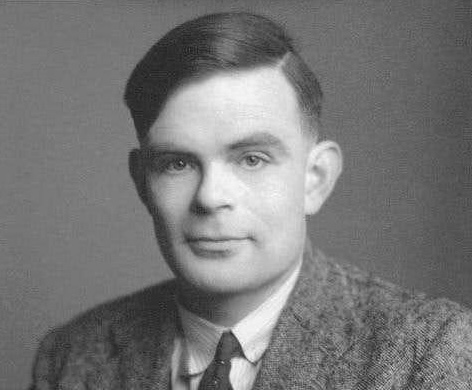
\includegraphics[width=4cm]{Photos/AlanTuring}};
			\end{tikzpicture}
		\end{column}
	\end{columns}
	
	\begin{itemize}
		\item \texthighlight{Conférence de Dartmouth - 1956} : Début des travaux dans l'objectif de créer des machines intelligentes
		\item \texthighlight{Scikit-Learn - 2007} : Création d'une librairie open-source pour faciliter la modélisation en Machine Learning
		\item \texthighlight{AlexNet - 2012} : avènement du Deep Learning avec un modèle de classification d'image révolutionnaire dans la compétition ImageNet
	\end{itemize}
\end{frame}

\begin{frame}{}{Qu'est-ce que \emph{l'Intelligence Artificielle} ?}
	
	\begin{columns}
		\begin{column}{0.6\textwidth}
			\begin{itemize}
				\item \texthighlight{Algorithme} : Ensemble hiérarchisé d'opérations logiques à exécuter dans le but de résoudre un problème\footnote{Aurélie Jean, De l'autre côté de la Machine}
				\item \texthighlight{Intelligence artificielle} : Ensemble d'algorithme résolvant des problèmes sans être explicitement programmé pour le faire
				\item \texthighlight{Machine Learning} : Sous-ensemble de l'IA où les algorithmes apprennent à partir d'une base de données
				\item \texthighlight{Deep Learning} : Sous-ensemble du ML où les algorithmes sont des variantes d'un algorithme de ML nommé \textit{réseau de neurones}
			\end{itemize}
		\end{column}
		
		\begin{column}{0.4\textwidth}
			\begin{figure}
				\centering
				\begin{tikzpicture}[scale=0.8]
					\draw[primary, very thick, rounded corners, fill=primary!10] (0, 0) rectangle (6, 9);
					\draw[secondary, very thick, rounded corners, fill=secondary!10] (0.5, 0.5) rectangle (5.5, 7);
					\draw[tertiary, very thick, rounded corners, fill=tertiary!10] (1, 1) rectangle (5, 5);
					\draw (3, 8) node[primary]{\textbf{Intelligence artificielle}};
					\draw (3, 6) node[secondary]{\textbf{Machine Learning}};
					\draw (3, 4) node[tertiary]{\textbf{Deep Learning}};
				\end{tikzpicture}
			\end{figure}
		\end{column}
	\end{columns}
\end{frame}



\begin{frame}{}{Formalisation : Dataset}
	Pour chacun, on peut considérer plusieurs approches, entre autres :
			
	\begin{itemize}
		\item \texthighlight{Supervisé} : on cherche à reproduire une réponse à partir de données
		\item \texthighlight{Non supervisé} : on ne possède pas de réponse pré-définie, on peut vouloir réduire la dimension, regrouper les observations qui se ressemblent...
		\item \texthighlight{Par renforcement} : on apprend la meilleure action à réaliser dans un environnement sur lequel on agit, selon une politique fixée\newline
	\end{itemize}
	
	Dans le cadre supervisé, nous avons accès à un dataset $\mathcal{D}$ défini comme :\newline
	
	\begin{equation*}
		\mathcal{D} = \left\{(x_i, y_i) \; | \; \forall i \leqslant \tikzmarknode{observations}{\highlight{secondary}{n}}, \; x_i \in \mathbb{R}^{\tikzmarknode{dimension}{\highlight{primary}{d'}}}, y_i \in \mathcal{Y}\right\}
	\end{equation*}\newline
	\begin{tikzpicture}[overlay, remember picture, >=stealth, nodes={align=left, inner ysep=1pt}, <-]
		\path (observations.south) ++ (0, -1em) node[anchor=north east, color=secondary!60] (observations_point){\textbf{Nombre d'observations}};
		 \draw [color=secondary!80](observations.south) |- ([xshift=-0.3ex, color=secondary] observations_point.north west);
		
		\path (dimension.north) ++ (0, 1.5em) node[anchor=north west, color=primary!60] (dimension_point){\textbf{Nombre d'informations}};
		 \draw [color=primary!80](dimension.north) |- ([xshift=-0.3ex, color=primary] dimension_point.south east);
	\end{tikzpicture}

	Avec $\mathcal{Y} \subseteq \mathbb{R}$ pour un problème de régression et $\mathcal{Y} \subset \mathbb{N}$ dans le cadre d'une classification. Dans le cadre non supervisé nous n'avons pas de $y$.
\end{frame}



\begin{frame}{}{Formalisation : Fonction de perte}
	Les problèmes de Machine Learning supervisé peuvent souvent s'écrire sous la forme d'une optimisation d'une fonction de perte $\displaystyle \mathcal{L}: \mathbb{R}^d\times\mathcal{M}_{n, d'}\times\mathbb{R}^n \rightarrow \mathbb{R}_+$ comme : \newline

	\begin{equation*}
		\tikzmarknode{theta_optimal}{\highlight{primary}{w^*}} = \argmin_{w\in\mathbb{R}^{\tikzmarknode{dimension_theta}{\highlight{secondary}{d}}}} \mathcal{L}(w, X, y)
	\end{equation*}
	\begin{tikzpicture}[overlay, remember picture, >=stealth, nodes={align=left, inner ysep=1pt}, <-]
		\path (theta_optimal.north) ++ (0, 2em) node[anchor=north east, color=primary!60] (theta_optimal_point){\textbf{Vecteur des paramètres optimaux}};
		 \draw [color=primary!80](theta_optimal.north) |- ([xshift=-0.3ex, color=primary] theta_optimal_point.south west);
	 
		\path (dimension_theta.south) ++ (0, -1em) node[anchor=north west, color=secondary!60] (dimension_theta_point){\textbf{Dimension du vecteur de paramètres}};
		 \draw [color=secondary!80](dimension_theta.south) |- ([xshift=-0.3ex, color=secondary] dimension_theta_point.north east);
	\end{tikzpicture}\newline

	Dans la suite, pour simplifier les notations, nous omettrons la dépendance de $\mathcal{L}$ en $X$ (matrice des informations) et $y$ (vecteur réponse). Notons qu'en général, nous avons $d\neq d'$ et dans le cas du deep learning, très souvent $d>>d'$.
\end{frame}







\section{Principaux algorithmes}



\subsection{Régression logistique}

\begin{frame}{}{}
	La régression logistique suppose un lien \textit{linéaire} entre les features et la côte que l'observation soit de la classe d'intérêt. On modélise cela par la fonction $f$ :
	
	\begin{equation*}
		f(x) = \frac{1}{\displaystyle 1+e^{\displaystyle-(x_1w_1 + \ldots + x_dw_d)}} = \frac{1}{\displaystyle 1+e^{\displaystyle-\langle x, \tikzmarknode{RLweight}{\highlight{secondary}{w}}\rangle}}
		\tag{Régression logistique}
	\end{equation*}

	\begin{tikzpicture}[overlay, remember picture, >=stealth, nodes={align=left, inner ysep=1pt}, <-]
		\path (RLweight.north) ++ (0em, -2em) node[anchor=north west, color=secondary!60] (RLweight_point) {$w = (w_1, \ldots, w_d)\in \mathbb{R}^d$};
		\draw [color=secondary!80] (RLweight.south) |- ([xshift=-0.3ex, color=secondary] RLweight_point.north east);
	\end{tikzpicture}

	
	\begin{figure}
		\centering
		\begin{tikzpicture}[scale=1, samples=200, domain=-3.5:3.5]
			\draw[->] (-3.5, 0) -- (3.5, 0) node[right]{$x$};
			\draw[->] (0, -0.5) -- (0, 3.75) node[above]{$f(x)$};
			\draw (0, 3.5) node[left]{$1$};
			\draw (0, 1.75) node[above left]{$0.5$};
			\draw[color=primary, thick] plot(\x, {3.5/(1+exp(-\x))});
			\draw[color=secondary, thick] plot(\x, {3.5/(1+exp(-2*\x))});
		\end{tikzpicture}
		\caption{${\color{primary}\displaystyle f(x)=\frac{1}{1+e^{-x}}}$ et ${\color{secondary}\displaystyle f(x)=\frac{1}{1+e^{-2x}}}$}
	\end{figure}	
\end{frame}


\begin{frame}{}{}
	Pour apprendre $w\in\mathbb{R}^d$, on se propose la fonction de perte :\newline\newline
	\begin{equation*}
		\mathcal{L}(w) = -\left[\tikzmarknode{true}{\highlight{primary}{y\ln\left\{f(x)\right\}}} + \tikzmarknode{false}{\highlight{secondary}{(1-y)\ln\left\{1-f(x)\right\}}}\right]
	\end{equation*}\\

	\begin{tikzpicture}[overlay, remember picture, >=stealth, nodes={align=left, inner ysep=1pt}, <-]
		\path (true.north) ++ (0, +1em) node[anchor=south east, color=primary!60] (true_point){\textbf{Observation positive}};
		\draw [color=primary!80](true.north) |- ([xshift=-0.3ex, color=primary] true_point.south west);
		\path (false.south) ++ (0, -1em) node[anchor=north west, color=secondary!60] (false_point){\textbf{Observation négative}};
		\draw [color=secondary!80](false.south) |- ([xshift=-0.3ex, color=secondary]false_point.north east);
	\end{tikzpicture}
	
	\begin{figure}[h!]
		\centering
		\begin{tikzpicture}[scale=0.7, samples=100]
			\draw[->, thick] (0, 0) -- (0, 5) node[above] {$-\ln\left\{f(x)\right\}$};
			\draw[->, thick] (0, 0) -- (6, 0) node[right] {$f(x)$};
			\draw (5, 0) node[below]{$1$}; \draw (0, 0) node[below]{$0$}; 
	
			\draw [domain=0.1:4.9, very thick, primary] plot(\x, {-ln(\x/5)}); 
		\end{tikzpicture}
		\hspace{0.25cm}
		\begin{tikzpicture}[scale=0.7, samples=100]
			\draw[->, thick] (0, 0) -- (0, 5) node[above] {$-\ln\left\{1 - f(x)\right\}$};
			\draw[->, thick] (0, 0) -- (6, 0) node[right] {$f(x)$};
			\draw (5, 0) node[below]{$1$}; \draw (0, 0) node[below]{$0$}; 
	
			\draw [domain=0.1:4.9, very thick, secondary] plot(\x, {-ln(1 - \x/5)}); 
		\end{tikzpicture}	
	\end{figure}
\end{frame}


\begin{frame}{}{Régression logistique : descente de gradient}
	La méthode la plus utilisée pour résoudre ce genre de problème est la descente de gradient :

			\begin{equation*}
				w_{t+1} = w_t - \tikzmarknode{learning_rate}{\highlight{primary}{\eta_t}} \nabla\mathcal{L}\left(w_t\right)
			\end{equation*}

			\begin{tikzpicture}[overlay, remember picture, >=stealth, nodes={align=left, inner ysep=1pt}, <-]
				\path (learning_rate.south) ++ (0, -1em) node[anchor=north west, color=primary!60] (learning_rate_point){\textbf{Learning rate}};
				 \draw [color=primary!80](learning_rate.south) |- ([xshift=-0.3ex, color=primary] learning_rate_point.north east);
			\end{tikzpicture}
	
	\begin{columns}
		\begin{column}{0.6\textwidth}
			Quand on travaille avec des grands datasets, le coût de calcul/temps est grand si l'on calcule $\nabla\mathcal{L}\left(w_t\right)$ pour la totalité de la base. On peut donc considérer d'autres approches :
			\begin{itemize}
				\item \texthighlight{Stochastique (SGD)} : on sélectionne au hasard une observation et on met à jour $w$
				\item \texthighlight{Stochastique par batch} : on sélectionne aléatoirement une partie de la base (batch) et on met à jour $w$ à chaque batch
			\end{itemize}
			De nombreux travaux portent sur l'accélération de cette méthode et la caractérisation de la vitesse de convergence des différents schémas.
		\end{column}
		
		\begin{column}{0.4\textwidth}
			\begin{figure}
				\centering
				\begin{tikzpicture}[scale=3, samples=200]
					\draw[->, thick] (-0.5, 0) -- (1.25, 0);
					\draw[->, thick] (0, -0.25) -- (0, 1.5);
			
					\draw[color=primary, thick, domain=-0.5:1.2, thick] plot(\x, {\x * \x});
					\draw[color=secondary, thick, domain=0.33:1, thick] plot(\x, {\x * \x});
			
					\draw[secondary] (1.00, 1.00) node{$\bullet$} node[right]{$w_0$}; \draw[secondary] (0.80, 0.64) node{$\bullet$} node[right]{$w_1$}; \draw[secondary] (0.64, 0.41) node{$\bullet$} node[right]{$w_2$}; \draw[secondary] (0.51, 0.26) node{$\bullet$} node[right]{$w_3$}; \draw[secondary] (0.41, 0.17) node{$\bullet$} node[below right]{$w_4$}; \draw[secondary] (0.33, 0.11) node{$\bullet$} node[above left]{$w_5$};
				\end{tikzpicture}
			\caption{Exemple d'une descente de gradient pour $f(x)=x^2$}
			\end{figure}
		\end{column}
	\end{columns}
\end{frame}



\subsection{Arbre de décision}

\begin{frame}{}{}
	On cherche à présent une fonction sous la forme suivante, où l'on cherche les partitions $P$ de l'espace :\newline\newline
	\begin{equation*}
		f_\theta(x) = \sum_{\tikzmarknode{Partition}{\highlight{primary}{P \in \theta}}} \tikzmarknode{Value}{\highlight{secondary}{\mu_P}} \mathds{1}_{\{x \in P\}}
	\end{equation*}

	\begin{tikzpicture}[overlay, remember picture, >=stealth, nodes={align=left, inner ysep=1pt}, <-]
		\path (Partition.south) ++ (0, -0.75em) node[anchor=north west, color=primary!60] (partition_point){\textbf{Partition de l'espace}};
		\draw [color=primary!80](Partition.south) |- ([xshift=-0.3ex, color=primary] partition_point.north east);
		\path (Value.north) ++ (0, +0.75em) node[anchor=south east, color=secondary!60] (value_point){\textbf{Probabilité de la classe d'intérêt dans la partition $P$}};
		\draw [color=secondary!80](Value.north) |- ([xshift=-0.3ex, color=secondary] value_point.south west);
	\end{tikzpicture}
	
	
	\begin{columns}
		\begin{column}{0.5\textwidth}
			\begin{figure}[h!]
				\centering
				\begin{tikzpicture}[scale=0.75]
					\draw[->, thick] (0, 0) -- (5.5, 0) node[right]{$x_1$};
					\draw[->, thick] (0, 0) -- (0, 5.5) node[above]{$x_2$};	
					\draw[very thick, primary] (0.5, 0.5) node{$\bullet$}; \draw[very thick, primary] (1, 1) node{$\bullet$}; \draw[very thick, primary] (0.5, 2.5) node{$\bullet$}; \draw[very thick, primary] (2, 5) node{$\bullet$}; \draw[very thick, primary] (4.5, 4.5) node{$\bullet$}; \draw[very thick, primary] (4.5, 4) node{$\bullet$}; \draw[very thick, primary] (5, 4) node{$\bullet$}; \draw[very thick, primary] (5, 3.5) node{$\bullet$};
					\draw[very thick, secondary] (1.5, 4) node{$\bullet$}; \draw[very thick, secondary] (2, 3.5) node{$\bullet$}; \draw[very thick, secondary] (2.5, 4) node{$\bullet$}; \draw[very thick, secondary] (2.5, 1.5) node{$\bullet$}; \draw[very thick, secondary] (3, 0.5) node{$\bullet$}; \draw[very thick, secondary] (3.5, 1) node{$\bullet$}; \draw[very thick, secondary] (4.5, 0.5) node{$\bullet$}; \draw[very thick, secondary] (4.5, 1.5) node{$\bullet$};
					\draw[very thick, tertiary] (1.25, 0) node[tertiary, below]{Séparation 1} -- (1.25, 5.5);
					\draw[very thick, tertiary] (1.25, 2.5) -- (5.5, 2.5); \draw (4, 2.25) node[tertiary, right]{Séparation 2};
					\draw[very thick, tertiary] (3.5, 2.5) -- (3.5, 5.5) node[tertiary, above]{Séparation 3};
					\draw[very thick, tertiary] (1.25, 4.5) -- (3.5, 4.5) node[tertiary, above left]{Séparation 4};
				\end{tikzpicture}
				\caption{Exemple de partitionnement de l'espace}
			\end{figure}
		\end{column}
		\begin{column}{0.5\textwidth}
			\begin{figure}[h!]
				\centering
				\begin{tikzpicture}[scale=0.75]
					\draw (2, 6.5) node{$x_1 \leqslant 2.5$};
					\draw[->, thin] (2, 6.25) -- (1, 5.25); \draw[primary, very thick, fill=primary!10] (0.75, 5) circle(0.5);
					\draw[->, thin] (2, 6.25) -- (3, 5.25); \draw (3.5, 5) node{$x_2 \leqslant 5$};
					\draw[->, thin] (3.5, 4.75) -- (2.5, 3.75); \draw[secondary, very thick, fill=secondary!10] (2.25, 3.5) circle(0.5);
					\draw[->, thin] (3.5, 4.75) -- (4.5, 3.75); \draw (5, 3.5) node{$x_1 \leqslant 7$};
					\draw[->, thin] (5, 3.25) -- (6, 2.25); \draw[primary, very thick, fill=primary!10] (6.25, 2) circle(0.5);
					\draw[->, thin] (5, 3.25) -- (4, 2.25); \draw (3.5, 2) node{$x_2 \leqslant 9$}; \draw[->, thin] (3.5, 1.75) -- (2.5, 0.75);
					\draw[secondary, very thick, fill=secondary!10] (2.25, 0.5) circle(0.5); \draw[->, thin] (3.5, 1.75) -- (4.5, 0.75);
					\draw[primary, very thick, fill=primary!10] (4.75, 0.5) circle(0.5);
				\end{tikzpicture}
				\caption{Arbre de décision associé au partitionnement}
				\label{fig:solution}
			\end{figure}
		\end{column}
	\end{columns}
\end{frame}


\subsection{Boosting}

\begin{frame}{}{}
	\begin{columns}
		\begin{column}{0.3\textwidth}
			Le principe du Boosting est de combiner plusieurs algorithmes les uns après les autres pour que chacun corrige les erreurs du précédent.\newline
			Les fonctions ${\color{primary}h}$ sont ce qu'on cherche à apprendre, et on prend très souvent des arbres. Les scalaires ${\color{primary}\gamma}$ sont appris pendant l'entraînement
		\end{column}
		
		\begin{column}{0.7\textwidth}
			\begin{figure}[h!]
				\centering
				\begin{tikzpicture}[scale=0.7]
					\draw[<-, very thick] (0, 0) -- (0, 10) node[above, thick]{Étape};
					\draw[densely dashed, thin] (12, 0) node[below]{Vrai valeur} -- (12, 10);
					\draw[densely dashed, thin] (1, 0) node[below]{Prédiction initiale} -- (1, 10);
					\draw[very thick, ->] (1, 10) -- (1, 8) -- (6, 8) -- (6, 6) -- (9, 6) -- (9, 4) -- (11, 4) -- (11, 2) -- (12, 2) -- (12, 0);
					\foreach \iteration in {0, ..., 4}{\draw (0, 9 - \iteration * 2) node[left]{$m = \iteration$};}
					\draw[<->, thick, secondary] (1.25, 8.5) -- (11.75, 8.5); \draw[thick, secondary] (6.5, 8.5) node[above]{$r_1^{(i)}$};
					\draw[<->, thick, primary] (1.25, 7.5) -- (5.75, 7.5); \draw[thick, primary] (3.5, 7.5) node[below]{$\gamma_1 h_1(x^{(i)})$};
					\draw[<->, thick, secondary] (6.25, 6.5) -- (11.75, 6.5); \draw[thick, secondary] (9, 6.5) node[above]{$r_2^{(i)}$};
					\draw[<->, thick, primary] (6.25, 5.5) -- (8.75, 5.5); \draw[thick, primary] (7.5, 5.5) node[below]{$\gamma_2 h_2(x^{(i)})$};
					\draw[<->, thick, secondary] (9.25, 4.5) -- (11.75, 4.5); \draw[thick, secondary] (10.5, 4.5) node[above]{$r_3^{(i)}$};
					\draw[<->, thick, primary] (9.25, 3.5) -- (10.75, 3.5); \draw[thick, primary] (10, 3.5) node[below]{$\gamma_3 h_3(x^{(i)})$};
					\draw[<->, thick, secondary] (11.25, 2.5) -- (11.75, 2.5); \draw[thick, secondary] (11.5, 2.5) node[above]{$r_4^{(i)}$};
					\draw[<->, thick, primary] (11.25, 1.5) -- (11.75, 1.5); \draw[thick, primary] (11.25, 1.5) node[below]{$\gamma_4 h_4(x^{(i)})$};
				\end{tikzpicture}
			\end{figure}
		\end{column}
	\end{columns}
\end{frame}




\section{Quels challenges dans la lutte contre la fraude ?}

\subsection{Déséquilibre de classe}

\begin{frame}{}{Déséquilibre de classe : Sur-échantillonnage}
	Une première méthode pour équilibrer le dataset est de dupliquer aléatoirement des observations de la classe minoritaire, jusqu'à ce qu'on atteigne la proportion de la classe minoritaire voulue {\color{secondary}$p_f$}.\newline
	
	\visible<3->{
	\begin{equation}
		\tikzmarknode{size_final_OV}{\highlight{secondary}{n_f}} = \tikzmarknode{size_initial_OV}{\highlight{primary}{n_i}} \frac{1-\tikzmarknode{proportion_initial_OV}{\highlight{primary}{p_i}}}{1-{\highlight{secondary}{p_f}}}
		\tag{Over sampling}
	\end{equation}

	\begin{tikzpicture}[overlay, remember picture, >=stealth, nodes={align=left, inner ysep=1pt}, <-]
		\path (size_initial_OV.north) ++ (0, +0.75em) node[anchor=south east, color=primary!60] (size_initial_OV_point) {\textbf{Taille initiale du dataset}};
		\draw [color=primary!80](size_initial_OV.north) |- ([xshift=-0.3ex, color=primary] size_initial_OV_point.south west);
		\path (size_final_OV.south) ++ (0, -0.75em) node[anchor=north east, color=secondary!60] (size_final_OV_point) {\textbf{Taille finale du dataset}};
		\draw [color=secondary!80](size_final_OV.south) |- ([xshift=-0.3ex, color=secondary] size_final_OV_point.north west);
		\path (proportion_initial_OV.north) ++ (0, +0.75em) node[anchor=south west, color=primary!60] (proportion_initial_OV_point) {\textbf{Proportion de la classe minoritaire initiale}};
		\draw [color=primary!80](proportion_initial_OV.north) |- ([xshift=-0.3ex, color=primary] proportion_initial_OV_point.south east);
	\end{tikzpicture}}
	
	\begin{columns}
		\begin{column}{0.5\textwidth}
			\visible<2->{
			\begin{figure}
				\centering
				\begin{subfigure}[t]{.45\linewidth}
					\centering
					\begin{tikzpicture}[scale=1]
						\draw[very thick, primary, fill=primary!25] (0, 0) rectangle (1, 4); 
						\draw[very thick, secondary, fill=secondary!25] (1.5, 0) rectangle (2.5, 1); 
					\end{tikzpicture}
					\caption{Situation initiale}
				\end{subfigure}
				\begin{subfigure}[t]{.45\linewidth}
					\centering
					\begin{tikzpicture}[scale=1]
						\draw[very thick, primary, fill=primary!25] (0, 0) rectangle (1, 4); 
						\draw[very thick, secondary, fill=secondary!25] (1.5, 0) rectangle (2.5, 4); 
					\end{tikzpicture}
					\caption{Situation finale}
				\end{subfigure}
				\caption{Illustration du sur-échantillonnage}
			\end{figure}}
		\end{column}
		
		\begin{column}{0.5\textwidth}
			\visible<4->{
			\begin{figure}
				\centering
				\begin{tikzpicture}[scale=4, samples=200]
					\draw[->, thick] (0, 0) -- (1, 0); \draw (0.5, 0) node[below]{${\color{secondary}{p_f}}$};
					\draw[->, thick] (0, 0) -- (0, 1.1); \draw (0, 0.5) node[left]{\rotatebox{90}{Évolution de {\color{secondary}$n_f$} (\%)}};
					\draw (1, 0) node[below]{0.5};
					\draw[densely dashed] (1, 0) -- (1, 1); 
					\draw[secondary] (0.02, 0) node{$\bullet$} node[below]{1\%}; \draw[secondary] (1, 0.98) node{$\bullet$} node[right]{98\%};
					\draw[primary] (0.2, 0) node{$\bullet$} node[below]{10\%}; \draw[primary] (1, 0.80) node{$\bullet$} node[right]{80\%};
					\draw[thick, color=secondary, domain=0.02:1] plot(\x, {(1-0.01)/(1-0.5*\x) - 1});
					\draw[thick, color=primary, domain=0.2:1] plot(\x, {(1-0.1)/(1-0.5*\x) - 1});
				\end{tikzpicture}
				\caption{Évolution de la taille du dataset final en fonction de la proportion finale de la classe minoritaire}
			\end{figure}}
		\end{column}
	\end{columns}
\end{frame}

\begin{frame}{}{Déséquilibre de classe : Sous-échantillonnage}
	Une deuxième méthode pour équilibrer le dataset est de supprimer aléatoirement des observations de la classe majoritaire, jusqu'à ce qu'on atteigne la proportion de la classe minoritaire voulue {\color{secondary}$p_f$}.\newline
	
	\visible<3->{
	\begin{equation}
		\tikzmarknode{size_final_UD}{\highlight{secondary}{n_f}} = \tikzmarknode{size_initial_UD}{\highlight{primary}{n_i}} \frac{\tikzmarknode{proportion_initial_UD}{\highlight{primary}{p_i}}}{{\highlight{secondary}{p_f}}}
		\tag{Under sampling}
	\end{equation}

	\begin{tikzpicture}[overlay, remember picture, >=stealth, nodes={align=left, inner ysep=1pt}, <-]
		\path (size_initial_UD.north) ++ (0, +1em) node[anchor=south east, color=primary!60] (size_initial_UD_point) {\textbf{Taille initiale du dataset}};
		\draw [color=primary!80](size_initial_UD.north) |- ([xshift=-0.3ex, color=primary] size_initial_UD_point.south west);
		\path (size_final_UD.south) ++ (0, -1em) node[anchor=north east, color=secondary!60] (size_final_UD_point) {\textbf{Taille finale du dataset}};
		\draw [color=secondary!80](size_final_UD.south) |- ([xshift=-0.3ex, color=secondary] size_final_UD_point.north west);
		\path (proportion_initial_UD.north) ++ (0, +1em) node[anchor=south west, color=primary!60] (proportion_initial_UD_point) {\textbf{Proportion de la classe minoritaire initiale}};
		\draw [color=primary!80](proportion_initial_UD.north) |- ([xshift=-0.3ex, color=primary] proportion_initial_UD_point.south east);
	\end{tikzpicture}}

	\begin{columns}
		\begin{column}{0.5\textwidth}
			\visible<2->{
			\begin{figure}
				\centering
				\begin{subfigure}[t]{.45\linewidth}
					\centering
					\begin{tikzpicture}[scale=1]
						\draw[very thick, primary, fill=primary!25] (0, 0) rectangle (1, 4); 
						\draw[very thick, secondary, fill=secondary!25] (1.5, 0) rectangle (2.5, 1); 
					\end{tikzpicture}
					\caption{Situation initiale}
				\end{subfigure}
				\begin{subfigure}[t]{.45\linewidth}
					\centering
					\begin{tikzpicture}[scale=1]
						\draw[very thick, primary, fill=primary!25] (0, 0) rectangle (1, 1); 
						\draw[very thick, secondary, fill=secondary!25] (1.5, 0) rectangle (2.5, 1); 
					\end{tikzpicture}
					\caption{Situation finale}
				\end{subfigure}
				\caption{Illustration du sous-échantillonnage}
			\end{figure}}
		\end{column}
		
		\begin{column}{0.5\textwidth}
			\visible<4->{
			\begin{figure}
				\centering
				\begin{tikzpicture}[scale=4, samples=200]
					\draw[->, thick] (0, 0) -- (1.1, 0); \draw (0.5, 0) node[above]{${\color{secondary}{p_f}}$};
					\draw[->, thick] (0, 0) -- (0, -1.1); \draw (0, -0.5) node[left]{\rotatebox{90}{Évolution de {\color{secondary}$n_f$} (\%)}};
					\draw (1, 0) node[above]{0.5};
					\draw[densely dashed] (1, 0) -- (1, -1); 
					\draw[secondary] (0.02, 0) node{$\bullet$} node[above]{1\%}; \draw[secondary] (1, -0.98) node{$\bullet$} node[right]{-98\%};
					\draw[primary] (0.2, 0) node{$\bullet$} node[above]{10\%}; \draw[primary] (1, -0.8) node{$\bullet$} node[right]{-80\%};
					\draw[thick, color=secondary, domain=0.02:1] plot(\x, {(0.01)/(0.5*\x) - 1});
					\draw[thick, color=primary, domain=0.2:1] plot(\x, {(0.1)/(0.5*\x) - 1});
				\end{tikzpicture}
				\caption{Évolution de la taille du dataset final en fonction de la proportion finale de la classe minoritaire}
			\end{figure}}
		\end{column}
	\end{columns}
\end{frame}



\subsection{Drifts : changements de distributions}

\begin{frame}{}{}
	Le monde des paiements change, et les fraudeurs aussi. On peut noter deux manière principales dont les mouvements se font :
	\begin{itemize}
		\item \texthighlight{Covariate shift} : La distribution des features change
		\item \texthighlight{Concept drift} : La relation entre la cible et les features change
	\end{itemize}
	
	\begin{columns}
		\begin{column}{0.5\textwidth}
			\begin{figure}
				\centering
				\begin{tikzpicture}[scale=3, samples=200, domain=0:1]
					\draw[->] (0, 0) -- (1.25, 0) node[right]{$x$};
					\draw[->] (0, 0) -- (0, 1.5) node[above]{$p(x)$};
					\draw[color=blue, thick] plot(\x, {-3*\x*\x+4*\x});
					\draw[color=red, thick] plot(\x, {-6*\x*\x+6*\x});
				\end{tikzpicture}
				\caption{Covariate shift : changement de distribution d'une feature}
			\end{figure}
		\end{column}
		
		\begin{column}{0.5\textwidth}
			\begin{figure}
				\centering
				\begin{tikzpicture}[scale=4, samples=200, domain=0:1]
					\draw[->] (0, 0) -- (1, 0) node[right]{$x$};
					\draw[->] (0, 0) -- (0, 1) node[above]{$y$};
					\draw[color=blue, thick] plot(\x, {1.1*tanh(1.5*\x});
					\draw[color=red, thick] plot(\x, {\x});
				\end{tikzpicture}
				\caption{Concept drift : changement de relation entre $x$ et $y$}
			\end{figure}
		\end{column}
	\end{columns}
\end{frame}


\subsection{Fléau de la dimension}

\begin{frame}{}{Motivation}
	\begin{columns}
		\begin{column}{0.6\textwidth}
			\begin{customquote}{Georg Cantor}{1877}
				Tant que vous ne m'aurez pas approuvé, je ne puis que dire : je le vois mais je ne le crois pas.
			\end{customquote}
		\end{column}
		\begin{column}{0.5\textwidth}
			\centering
			\begin{tikzpicture}
				\clip (0,0) circle (1.75cm) node {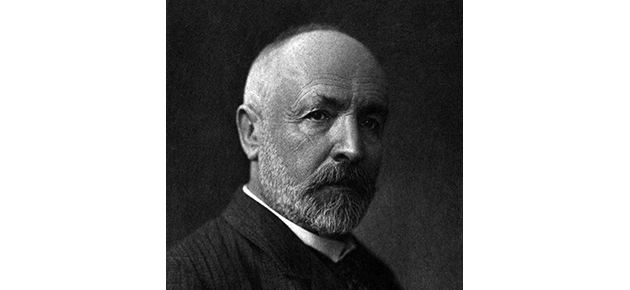
\includegraphics[width=8cm]{Photos/Cantor}};
			\end{tikzpicture}
		\end{column}
	\end{columns}
\end{frame}

\begin{frame}{}{Volume d'une hypersphère}
	\begin{figure}[h!]
		\centering
		\visible<1->{
		\begin{subfigure}[t]{.31\linewidth}
			\centering
			\begin{tikzpicture}[scale=0.5]
				\draw[primary, very thick] (-2, 0) node[primary, very thick]{$\bullet$} -- (2, 0) node[primary, very thick]{$\bullet$};
			\end{tikzpicture}
			\caption{En dimension 1, volume = 2}
		\end{subfigure}}
		\visible<2->{
		\begin{subfigure}[t]{.31\linewidth}
			\centering
			\begin{tikzpicture}[scale=0.5]
				\draw[primary, very thick] (0, 0) circle(2);
			\end{tikzpicture}
			\caption{En dimension 2, volume = $\pi$}
		\end{subfigure}}
		\visible<4->{
		\begin{subfigure}[t]{.31\linewidth}
			\centering
			\begin{tikzpicture}[scale=0.5]
  				\draw[primary, very thick] (0,0) circle (2);
  				\draw[primary, thick] (-2, 0) arc (180:360:2 and 0.6);
  				\draw[dashed, primary, thick] (2, 0) arc (0:180:2 and 0.6);
			\end{tikzpicture}
			\caption{En dimension 3, volume = $\frac{4}{3}\pi$}
		\end{subfigure}}
		\visible<1->{
		\caption{Représentation et volume d'une hypersphère de rayon 1 dans 3 espaces de dimensions différentes}}
	\end{figure}
	
	\begin{figure}[h!]
		\centering
		\visible<3->{
		\begin{subfigure}[t]{.31\linewidth}
			\centering
			\begin{tikzpicture}[scale=0.5]
				\draw[primary, very thick] (-2, 0) -- (0, -2) -- (2, 0) -- (0, 2) -- cycle;
			\end{tikzpicture}
			\caption{Avec la norme 1}
		\end{subfigure}}
		\visible<2->{
		\begin{subfigure}[t]{.31\linewidth}
			\centering
			\begin{tikzpicture}[scale=0.5]
				\draw[primary, very thick] (0, 0) circle(2);
			\end{tikzpicture}
			\caption{Avec la norme 2}
		\end{subfigure}}
		\visible<3->{
		\begin{subfigure}[t]{.31\linewidth}
			\centering
			\begin{tikzpicture}[scale=0.5]
  				\draw[primary, very thick] (-2, 2) -- (-2, -2) -- (2, -2) -- (2, 2) -- cycle;
			\end{tikzpicture}
			\caption{Avec la norme infinie}
		\end{subfigure}}
		\visible<2->{
		\caption{Représentation d'une hypersphère de rayon 1 en dimension 2 pour 3 normes différentes}}
	\end{figure}
\end{frame}

\begin{frame}{}{Volume d'une hypersphère}
	On appelle \textit{boule} ou hypersphère l'objet défini par :
	\begin{equation*} 
		B_n^p(R) = \{ u \in \mathbb{R}^n, \|u\|_p^p \leqslant R^p\}
	\end{equation*}
	
	Et son volume par :
	\begin{equation*} V_n^p(R) = \int_{B_n^p(R)} \bigotimes_{i=1}^n\mathrm{d}x_i \end{equation*}
	
	\begin{proposition}[Volume d'une hypersphere] Avec les notations précédentes, on a:
		\begin{eqnarray*} 
			\forall R>0, \forall n\geqslant 2, \forall p\geqslant 1, \; \; \; V_n^p(R) &=& \frac{\left(2R\Gamma\left(\frac{1}{p}+1\right)\right)^n}{\Gamma\left(\frac{n}{p}+1\right)} \\
			&\sim& \sqrt{\frac{p}{2\pi n}} \left[2R\Gamma\left(\frac{1}{p}+1\right) \left(\frac{pe}{n}\right)^{\frac{1}{p}}\right]^n 
		\end{eqnarray*}
	
		Avec la fonction $\Gamma$ définie comme :
		\begin{equation*} \Gamma(x) = \int_0^{+\infty} e^{-t}t^{x-1}\mathrm{d}t \end{equation*}
	\end{proposition}
\end{frame}



\begin{frame}{}{Concentration dans une hypersphère}
	On rappelle que :
	
	\begin{equation*}
		\forall R>0, \forall n\geqslant 2, \forall p\geqslant 1, \; \; \; V_n^p(R) = \frac{\left(2R\Gamma\left(\frac{1}{p}+1\right)\right)^n}{\Gamma\left(\frac{n}{p}+1\right)} 
	\end{equation*}
	
	\begin{exercice}[Concentration dans l'hypersphère]
		Soit $\varepsilon > 0$. On considère une hypersphère de rayon $R$. Montrer que :
			\begin{equation*} 
				\frac{V_n^p(R - \varepsilon)}{V_n^p(R)} = \left(1- \frac{\varepsilon}{R}\right)^n 
			\end{equation*}
	\end{exercice}
\end{frame}


\begin{frame}{}{En résumé}
	\begin{itemize}
		\item \texthighlight{L'hyper déséquilibre} de classe induit des difficultés d'entraînement et nécessite des réponses mesurées
		\item \texthighlight{Les drifts} inhérent à l'activité de production accentuent le premier point et nécessite une création et un suivi minutieux des algorithmes
		\item \texthighlight{Le fléau de la dimension} peut survenir plus tôt que prévu, une réponse est de mettre l'accent sur le travail métier pour créer de la valeur
	\end{itemize}
\end{frame}


%\begin{frame}[allowframebreaks]{Bibliographie}
%	\bibliographystyle{apalike}
%	\bibliography{Bibli_RecentAdvances}
%\end{frame}

%\appendix

\section{Annexe : SMOTE}
\begin{frame}{}{Fonctionnement}
	Les deux précédentes approches dupliquent ou suppriment des observations du dataset. On peut explorer la possibilité de \textit{créer} des observations synthétiques : c'est l'objet de SMOTE.
	
	\begin{figure}[h!]
		\centering
		\begin{subfigure}[t]{.32\linewidth}
			\centering
			\begin{tikzpicture}[scale=0.5, samples=100]
				\draw (1, 1) node[primary!50]{$\bullet$}; \draw (2, 2) node[primary!50]{$\bullet$}; \draw (3, 4) node[primary!50]{$\bullet$}; \draw (7, 5) node[primary!50]{$\bullet$}; \draw (5, 5) node[primary!50]{$\bullet$}; \draw (8, 2) node[primary!50]{$\bullet$}; \draw (7, 0) node[primary!50]{$\bullet$}; \draw (2, -1) node[primary!50]{$\bullet$}; \draw (3, 0) node[primary!50]{$\bullet$}; \draw (5, -2) node[primary!50]{$\bullet$};\draw (3, -2) node[primary!50]{$\bullet$}; \draw (7, -1) node[primary!50]{$\bullet$}; \draw (9, 0) node[primary!50]{$\bullet$}; \draw (5, 3) node[primary!50]{$\bullet$}; \draw (6, 3) node[primary!50]{$\bullet$}; \draw (7, 4) node[primary!50]{$\bullet$}; \draw (4, 2) node[primary!50]{$\bullet$}; \draw (4, -1) node[primary!50]{$\bullet$};
			\draw[secondary, thick] (5, 2) circle(0.35);
			\draw (1, 3) node[secondary!50]{$\bullet$}; \draw (5, 2) node[secondary]{$\bullet$}; \draw (6, 2) node[secondary!50]{$\bullet$}; \draw (6, 1) node[secondary!50]{$\bullet$}; \draw (3, 1) node[secondary!50]{$\bullet$}; \draw (8, 1) node[secondary!50]{$\bullet$}; \draw (5, 0) node[secondary!50]{$\bullet$}; \draw (4, 3) node[secondary!50]{$\bullet$};
			\end{tikzpicture}
			\caption{Sélection aléatoire d'une observation de la classe minoritaire}
		\end{subfigure}
		\begin{subfigure}[t]{.32\linewidth}
			\centering
			\begin{tikzpicture}[scale=0.5, samples=100]
				\draw (1, 1) node[primary!50]{$\bullet$}; \draw (2, 2) node[primary!50]{$\bullet$}; \draw (3, 4) node[primary!50]{$\bullet$}; \draw (7, 5) node[primary!50]{$\bullet$}; \draw (5, 5) node[primary!50]{$\bullet$}; \draw (8, 2) node[primary!50]{$\bullet$}; \draw (7, 0) node[primary!50]{$\bullet$}; \draw (2, -1) node[primary!50]{$\bullet$}; \draw (3, 0) node[primary!50]{$\bullet$}; \draw (5, -2) node[primary!50]{$\bullet$};\draw (3, -2) node[primary!50]{$\bullet$}; \draw (7, -1) node[primary!50]{$\bullet$}; \draw (9, 0) node[primary!50]{$\bullet$}; \draw (5, 3) node[primary!50]{$\bullet$}; \draw (6, 3) node[primary!50]{$\bullet$}; \draw (7, 4) node[primary!50]{$\bullet$}; \draw (4, 2) node[primary!50]{$\bullet$}; \draw (4, -1) node[primary!50]{$\bullet$};
			\draw[secondary, densely dashed, thick] (5, 2) circle(2.23);
			\draw[secondary, densely dashed] (5, 0) -- (5, 2); \draw[secondary, densely dashed] (4, 3) -- (5, 2); \draw[secondary, densely dashed] (6, 2) -- (5, 2); \draw[secondary, densely dashed] (6, 1) -- (5, 2); \draw[secondary, densely dashed] (3, 1) -- (5, 2);
			\draw (1, 3) node[secondary!50]{$\bullet$}; \draw (5, 2) node[secondary]{$\bullet$}; \draw (6, 2) node[secondary]{$\bullet$}; \draw (6, 1) node[secondary]{$\bullet$}; \draw (3, 1) node[secondary]{$\bullet$}; \draw (8, 1) node[secondary!50]{$\bullet$}; \draw (5, 0) node[secondary]{$\bullet$}; \draw (4, 3) node[secondary]{$\bullet$};
			\end{tikzpicture}
			\caption{Identification des $k$=5 voisins les plus proches}
		\end{subfigure}
		\begin{subfigure}[t]{.32\linewidth}
			\centering
			\begin{tikzpicture}[scale=0.5, samples=100]
				\draw (1, 1) node[primary!50]{$\bullet$}; \draw (2, 2) node[primary!50]{$\bullet$}; \draw (3, 4) node[primary!50]{$\bullet$}; \draw (7, 5) node[primary!50]{$\bullet$}; \draw (5, 5) node[primary!50]{$\bullet$}; \draw (8, 2) node[primary!50]{$\bullet$}; \draw (7, 0) node[primary!50]{$\bullet$}; \draw (2, -1) node[primary!50]{$\bullet$}; \draw (3, 0) node[primary!50]{$\bullet$}; \draw (5, -2) node[primary!50]{$\bullet$};\draw (3, -2) node[primary!50]{$\bullet$}; \draw (7, -1) node[primary!50]{$\bullet$}; \draw (9, 0) node[primary!50]{$\bullet$}; \draw (5, 3) node[primary!50]{$\bullet$}; \draw (6, 3) node[primary!50]{$\bullet$}; \draw (7, 4) node[primary!50]{$\bullet$}; \draw (4, 2) node[primary!50]{$\bullet$}; \draw (4, -1) node[primary!50]{$\bullet$};
			\draw[secondary, densely dashed] (5, 2) -- (5, 0);
			\draw[secondary, thick] (5, 1.2) circle(0.35);
			\draw (1, 3) node[secondary!50]{$\bullet$}; \draw (5, 2) node[secondary]{$\bullet$}; \draw (6, 2) node[secondary!50]{$\bullet$}; \draw (6, 1) node[secondary!50]{$\bullet$}; \draw (3, 1) node[secondary!50]{$\bullet$}; \draw (8, 1) node[secondary!50]{$\bullet$}; \draw (5, 0) node[secondary]{$\bullet$}; \draw (4, 3) node[secondary!50]{$\bullet$};\draw (5, 1.2) node[secondary]{$\bullet$};
			\end{tikzpicture}
			\caption{Sélection aléatoire d'un voisin et création de l'observation}
		\end{subfigure}
		\caption{Fonctionnement de SMOTE}
	\end{figure}
\end{frame}



\begin{frame}{}{Observations synthétiques ambiguës}
	
	Soit $\mathcal{D}$ un dataset comme défini dans l'introduction dont on reprend les notations, et $\mathcal{D}^-$ le dataset contenant uniquement les observations de la classe majoritaire. On note $n^- = \#\mathcal{D}^-$.\\
	Soit $\widetilde{x}$ un point synthétique généré par l'algorithme SMOTE. On dit que $\widetilde{x}$ est un \textbf{point ambigu} si $\displaystyle \min_{x\in \mathcal{D}^-} \|\widetilde{x}-x\| \leqslant \delta$ pour $\delta \geqslant 0$ un paramètre fixé.\\
	
	On peut montrer, sous l'hypothèse que $\mathcal{D}\sim\mathcal{N}(0_d, I_d)$, que :
	
	\begin{equation*}
		\probability{\min_{x\in \mathcal{D}^-} \|\widetilde{x}-x\| \leqslant \delta} = 1 - \left(1 - \int_0^{\frac{\delta^2}{2}} \frac{t^{\frac{d}{2}-1}e^{-\frac{t}{2}}}{2^{\frac{d}{2}}\Gamma\left(\frac{d}{2}\right)} \mathrm{d}t \right)^{n^-}
	\end{equation*}
	
	Ainsi, plus $n^-$ est grand, plus la probabilité de créer des observations synthétiques ambiguës est importante. Il faut également noter que quand $d$ tend vers l'infini, la probabilité tend vers 0 : mais ce régime n'est pas souhaitable avec le fléau de la dimension.
\end{frame}



\begin{frame}{}{Observations synthétiques ambiguës - observation sur un dataset réel}
	Nous souhaitons appliquer cela à un dataset de 20 millions de lignes ayant 1\% de déséquilibre. \newline
	
	\begin{table}
		\centering
		\begin{tabular}{@{}ccc@{}}\toprule
			Déséquilibre final (\%) & Observation synthétique ambiguë (\%) & Taille du dataset final (en millions)\\ \midrule
			1 & 0 & 20.000\\
			2 & 39.29 & 20.204\\
			5 & 62.86 & 20.842\\
			10 & 70.72 & 22.000\\
			20 & 74.65 & 24.750\\
			30 & 75.96 & 28.285\\
			40 & 76.61 & 33.000\\
			50 & 77.01 & 39.600\\ \bottomrule
		\end{tabular}
		\caption{Évolution de la proportion d'observation synthétique ambiguë et de la taille du dataset final en fonction de la proportion de déséquilibre souhaité}
	\end{table}
	
	Nous avons fixé la valeur de $\delta$ comme le quantile à 0.5\% de la loi du $\chi^2$ induite par le dataset.
\end{frame}


\end{document}